\chapter{General Context}
\section*{Introduction}
In this chapter, we will put the project named "\textbf{Auto Handover}" in its general context.
% Une section

% Exemple d'une section qui porte une référence à une bibliographie
% NB: il faut bien suivre le syntaxe pour ne pas tomber dans le cas où il y a une référence dans la table des matières.
\section{Project context}

Our project revolves around automating a multitude of tasks done manually by the Linedata support team, and bundling them into a Web Application.

\section{Problem}

The Linedata support team does Handovers
\footnote{A process done by a support team in which it passes a report to another team starting 
a new shift to make them aware of occuring changes (will be expanded upon in upcoming chapters)} 
and Checks
\footnote{Manual client application middle tier checks to test if it is up and running as expected (will be expanded upon in upcoming chapters)} 
tasks every day, which is time consuming, therefore hindering productivity, so any time saved doing these 
tasks will make the team answer more client calls and/or have more time investigating client problems.


\section[Host Organisation]{Host Organisation: Linedata Tunisie}
\textbf{Linedata} is a software editor, developping solutions mainly directed to the financial sector 
and providing a multitude of other related services; Data analytics, Advisory... to list a few\cite{LinedataAboutUs}.
% NB: il faut annoncer la figure dabord.
% Pour faire appel à une figure, il suffit d'utiliser le label comme suit :
% La figure \ref{fig:logo_tt} présente le logo de la tunisie télécom. (Il est déconseillé de mettre le logo de la société dans le rapport, il est déjà présent dans la page de garde).

% On peut ajouter une figure en utilisant le schapteryntaxe suivant:
% \begin{figure}[htpb]
% \centering
% \frame{
\includegraphics[width=0.5\columnwidth]{Logo_Entreprise}}
% \caption{Logo Entreprise}
% \label{fig:logo_tt}
% \end{figure}
\section{Proposed solution and global objectives}

Our main goals are:
\begin{itemize}
    \item Implementing a middle tier checking module that gets the status of a client application server
    \item generating reports and sending the output via SMTP
\end{itemize}
In light of the previously mentioned goals we proposed an intuitive web interface that includes configuration
options and a dashboard.

% \section{Etude bibliographique (sur un thème précis)}

% \section{Solution proposée et objectifs globaux du projet}

\section{Project management}
Making a project means to also manage its allocated resources efficiently in order to delivier a quality 
service within the deadline.\\
\textbf{Classical} and \textbf{Agile} methodologies exist; So choosing a proper project management methodology is critical.

Based on the fact that our project's needs are ever changing, we have chosen to work with \textbf{Agile} project management.
\subsection{XP: Extreme Programming}
Extreme programming is a popular agile framework which is conceived to address software development needs
within a small team, usually in pairs; to do extensive code reviewings and unit testing, mainting a high client involvement. \cite{XPIntro}\\
\begin{figure}[htpb]
\centering
\frame{
\includegraphics[width=0.5\columnwidth]{Extreme_Programming.svg.png}}
\caption{Extreme Programming process \cite{WikiXP}}
\label{fig:XP_process}
\end{figure}

\subsection{Scrum}
Among the main \textbf{Agile} project management methodologies, \textbf{Scrum} is quite the most known within
the software engineering communities and even incorporated in other projects not even related to software
development.
\begin{quote}
    "\textbf{Scrum} is a lightweight framework that helps people, teams and organizations generate value through adaptive solutions for complex problems." \cite{WhatIsScrum}
\end{quote}
\textbf{Scrum}'s simple and offers alot of flexibility with its easy to understand rules and few actors (see \ref{fig:Scrum_process}).
 
\subsubsection*{Scrum artifacts:}
\begin{itemize}
    \item \textbf{Product backlog}: A list of the desired product's functionalities.
    \item \textbf{Sprint backlog}: A list of short term goals for a sprint.
    \item \textbf{Product increment}: A shippable version of the product outputted at the end of each sprint.
\end{itemize}

\begin{figure}[htpb]
    \centering
    \frame{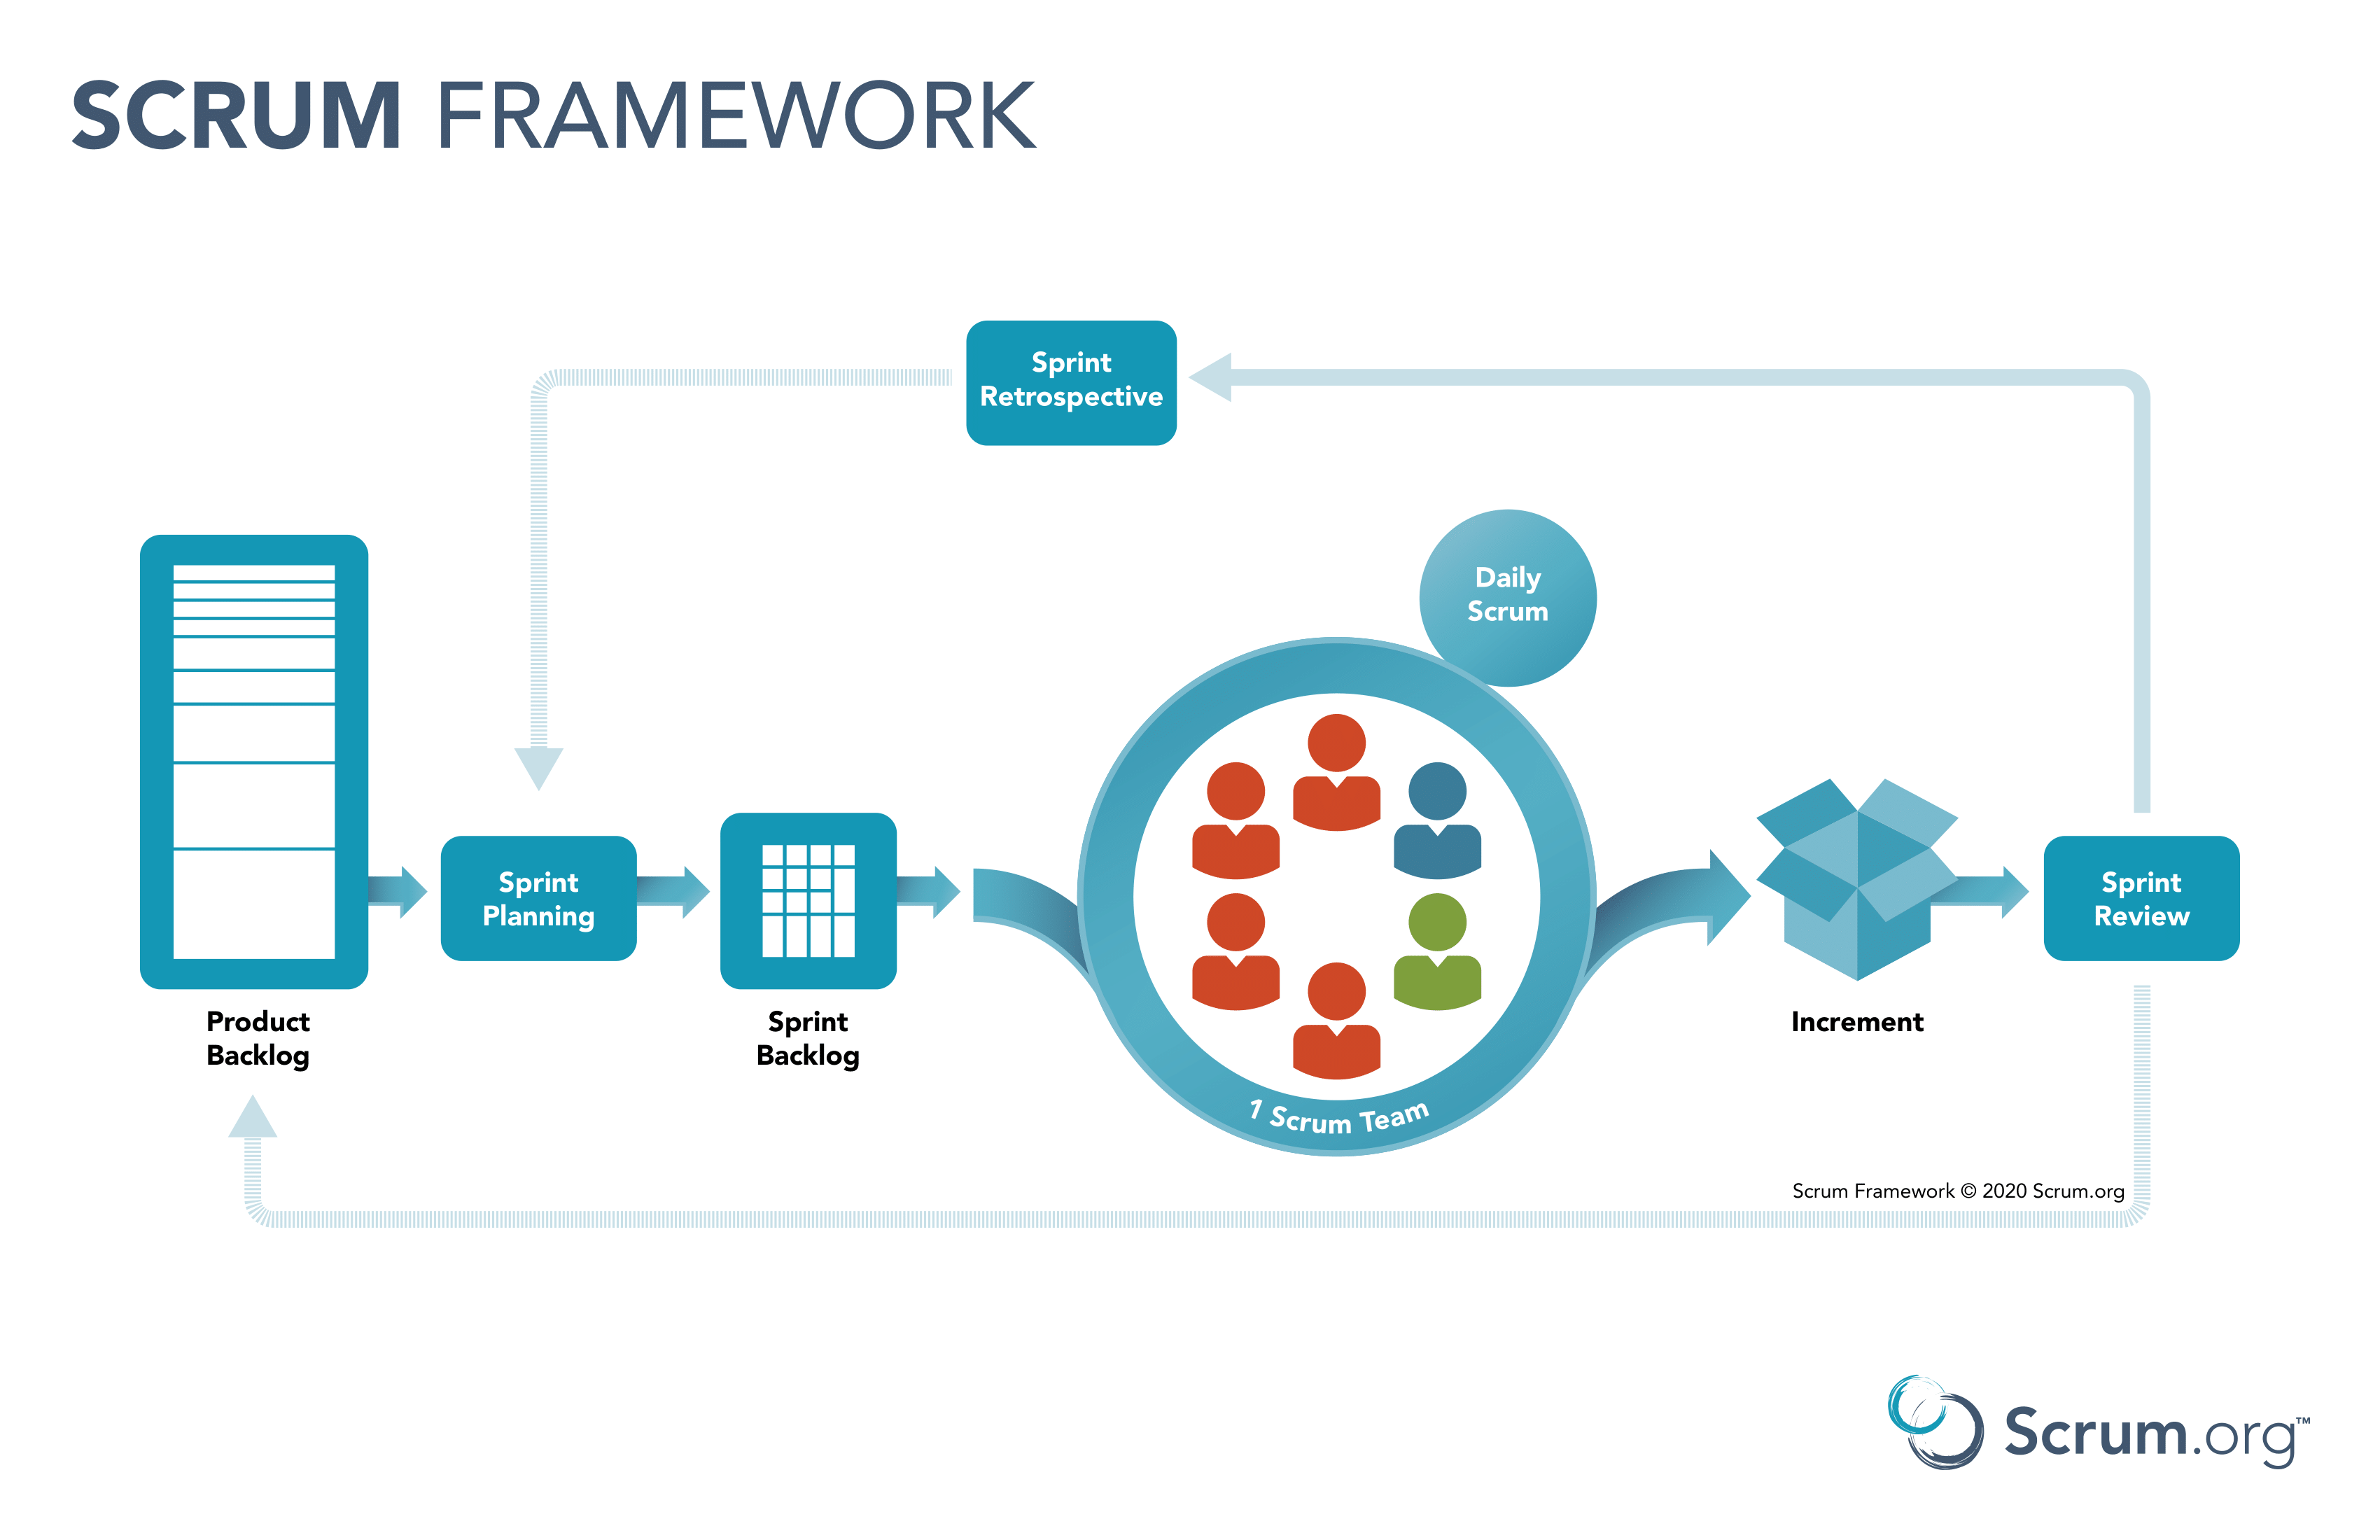
\includegraphics[width=1\columnwidth]{Scrumorg-Scrum-Framework-tabloid-1.png}}
    \caption{The Scrum process \cite{ScrumPoster}}
    \label{fig:Scrum_process}
    \end{figure}

We adopted the main ideology of agile development; Involving the client as frequently as possible, shipping iterations,
and using the Scrum artifacts, backlogging what needs to be done in each iteration.

% Le tableau \ref{tab:myfirstlongtable}
% \begin{longtable}[c]{
%     |p{.20\textwidth}
%     |p{.60\textwidth}|
% }
%     \caption{Some Data}
%     \label{tab:myfirstlongtable}\\
%     \hline
    
%     0
%     & 0 \\
%     \hline 
    
%     1
%     & 1 \\
%     \hline 
    
%     2
%     & 2 \\
%     \hline
% \end{longtable}

\section*{Conclusion}
We have presented a general idea about the set of our project, In next chapter We will address the 
technologies and planning of the project.